\documentclass[sigplan,review,anonymous]{acmart}
\setcopyright{none}
\settopmatter{printfolios=true,printacmref=false,printccs=false}
\renewcommand\footnotetextcopyrightpermission[1]{}
\def\shorttitle{AegisKV SGLSim Figure Insertion Proof}
\def\shortauthors{Anonymous}
\pagestyle{plain}
\usepackage{graphicx}
\microtypesetup{expansion=false}
\graphicspath{{figures/}}

\begin{document}
\typeout{AEGISKV_TEXTWIDTH=\the\textwidth}
\typeout{AEGISKV_COLUMNWIDTH=\the\columnwidth}

\begin{figure*}[p]
  \centering
  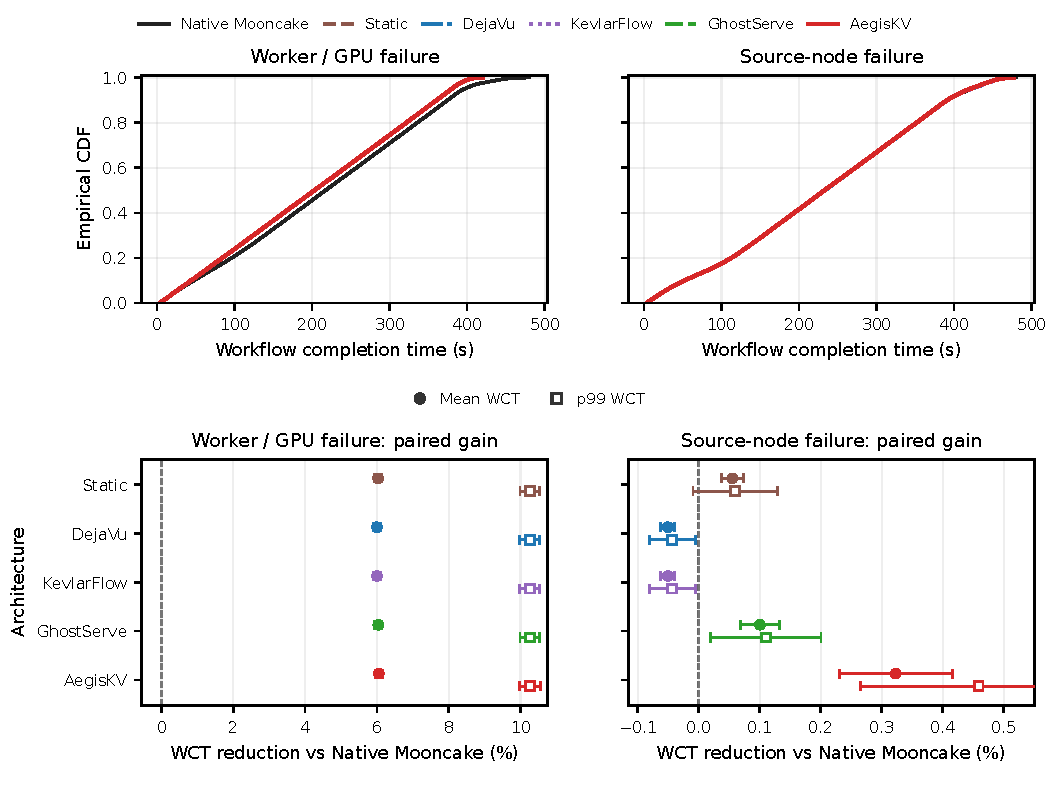
\includegraphics[width=\textwidth]{s1.pdf}
  \Description{Modeled WCT distributions for six architectures and two failure domains.}
  \caption{\textbf{S1.} Modeled WCT distributions for six architectures and two failure domains. Worker fault gains are dominated by avoiding the shared 60 s Native replacement; node faults also lose local replicas. Ten paired seeds; A100-40GiB metadata DES.}
\end{figure*}
\clearpage

\begin{figure*}[p]
  \centering
  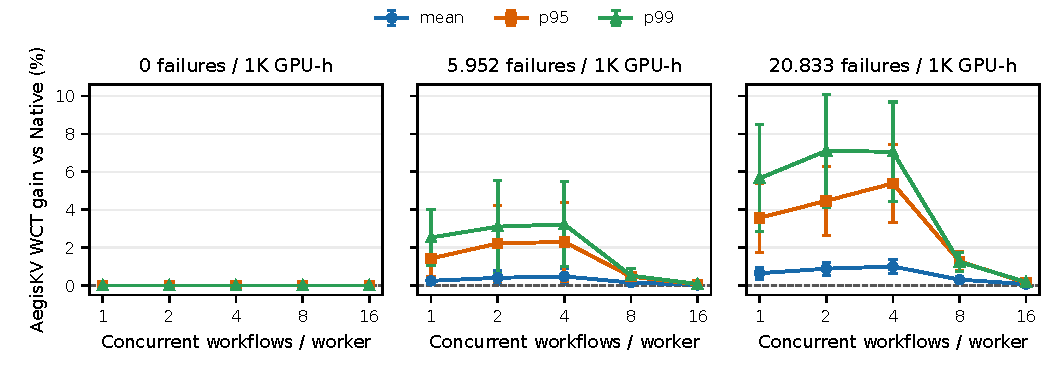
\includegraphics[width=\textwidth]{s2.pdf}
  \Description{AegisKV WCT reduction versus Native Mooncake over concurrency and failure rate.}
  \caption{\textbf{S2.} AegisKV WCT reduction versus Native Mooncake over concurrency and failure rate. Benefits peak at moderate load and collapse at C=8/16 as pressure reaches 100 percent and Peer-HBM protection approaches zero. Ten paired seeds.}
\end{figure*}
\clearpage

\begin{figure*}[p]
  \centering
  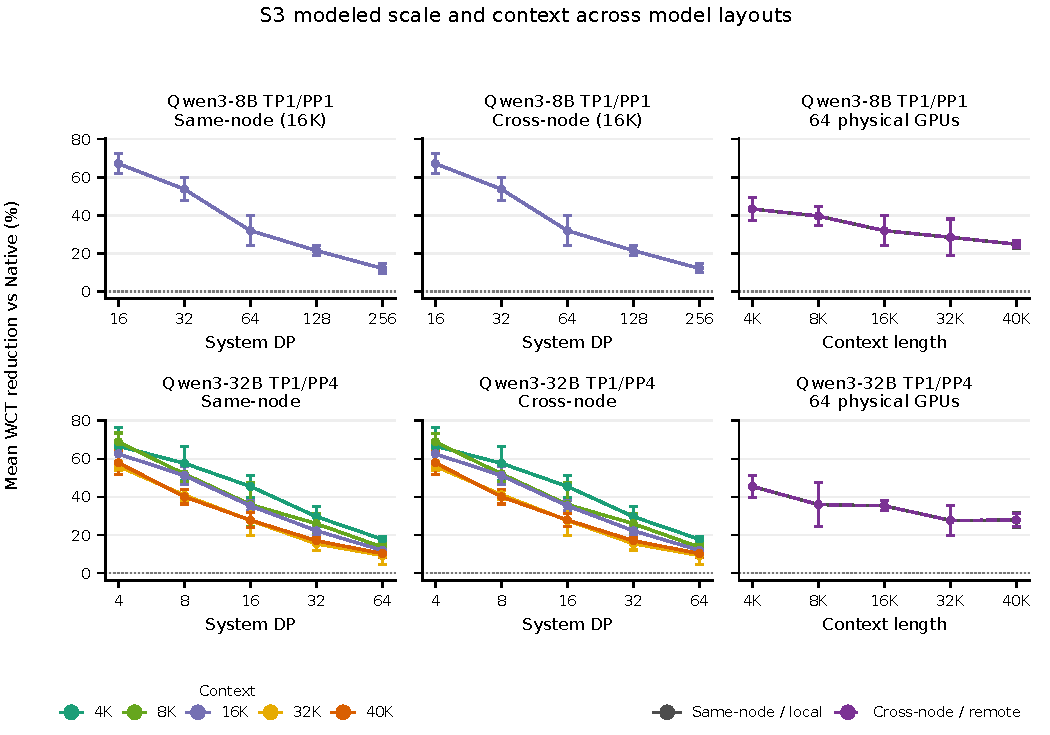
\includegraphics[width=\textwidth]{s3.pdf}
  \Description{Modeled scale and context sensitivity for Qwen3-8B and Qwen3-32B.}
  \caption{\textbf{S3.} Modeled scale and context sensitivity for Qwen3-8B TP1/PP1 and Qwen3-32B TP1/PP4. Fixed probes per cell dilute all-workflow gains as DP grows; the 32B service profile and failover delays are analytic rather than A100 measurements.}
\end{figure*}
\clearpage

\begin{figure*}[p]
  \centering
  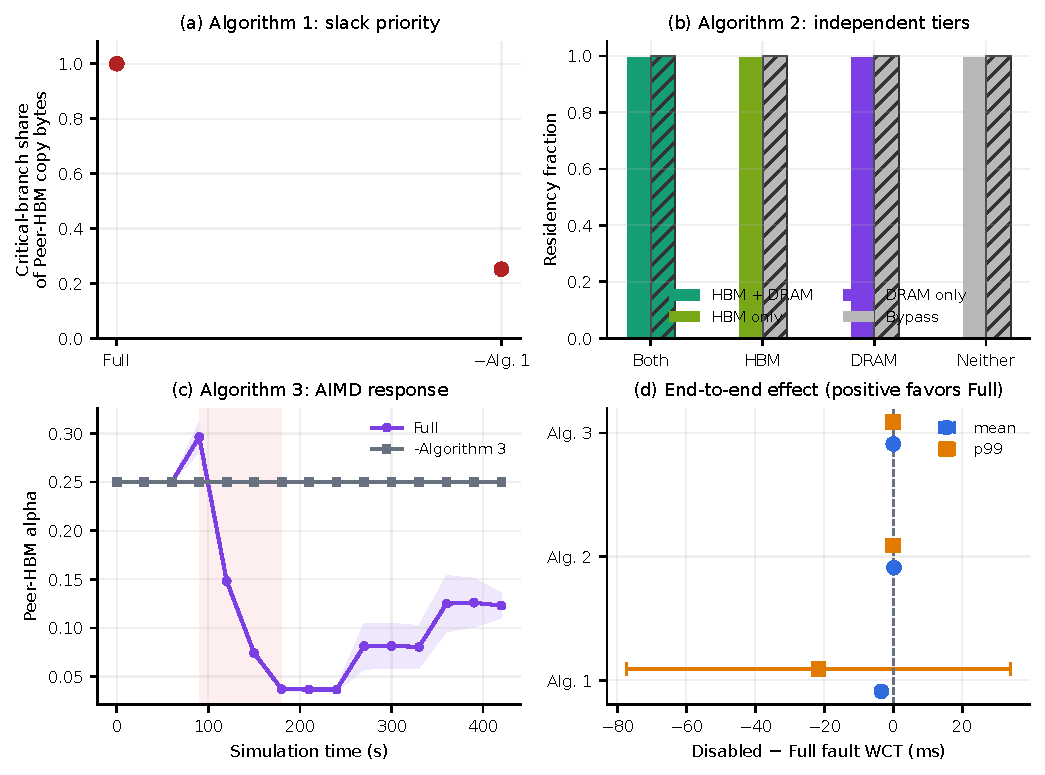
\includegraphics[width=\textwidth]{s4.pdf}
  \Description{Algorithms 1-3 mechanism ablations and paired end-to-end WCT effects.}
  \caption{\textbf{S4.} Algorithms 1-3 mechanism ablations. Slack priority, independent-tier outcomes, and AIMD behavior separate cleanly, while paired end-to-end WCT effects remain weak or negative. All three paired seeds and confidence intervals are retained.}
\end{figure*}
\clearpage

\begin{figure*}[p]
  \centering
  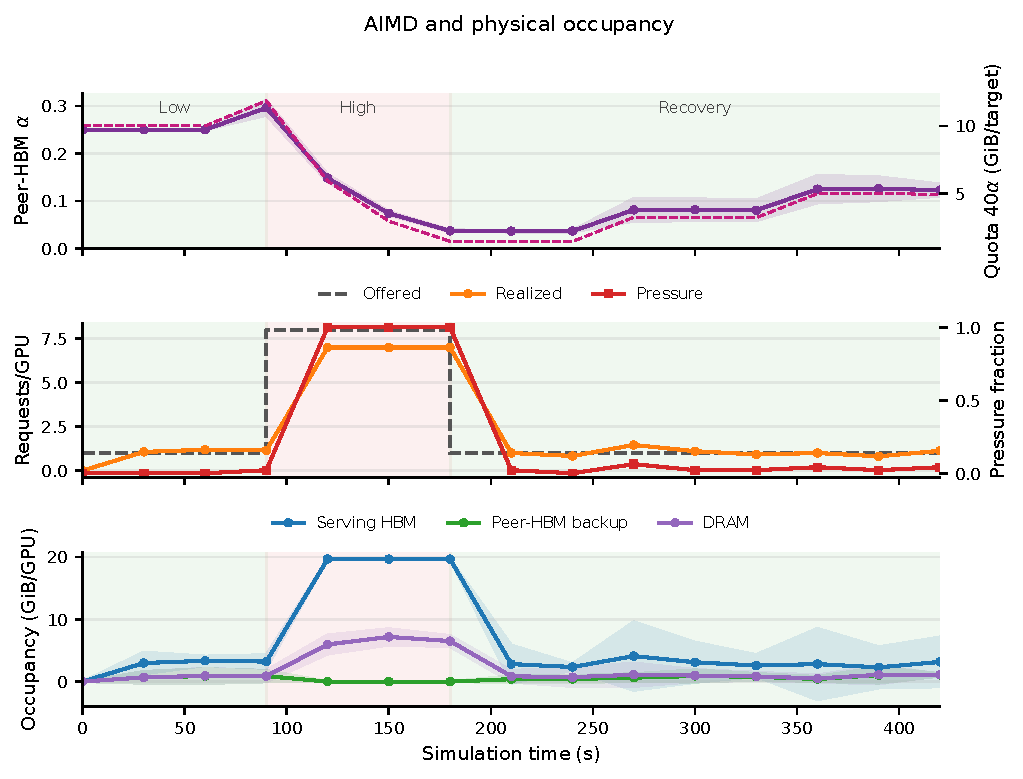
\includegraphics[width=\textwidth]{s5.pdf}
  \Description{AIMD and occupancy under low, high, and recovery phases.}
  \caption{\textbf{S5.} AIMD and occupancy under low, high, and recovery phases. Alpha contracts to about 0.037 and later recovers to about 0.125; residual pressure explains the nonmonotonic windows. Three-seed A100-40GiB metadata DES.}
\end{figure*}
\clearpage

\begin{figure*}[p]
  \centering
  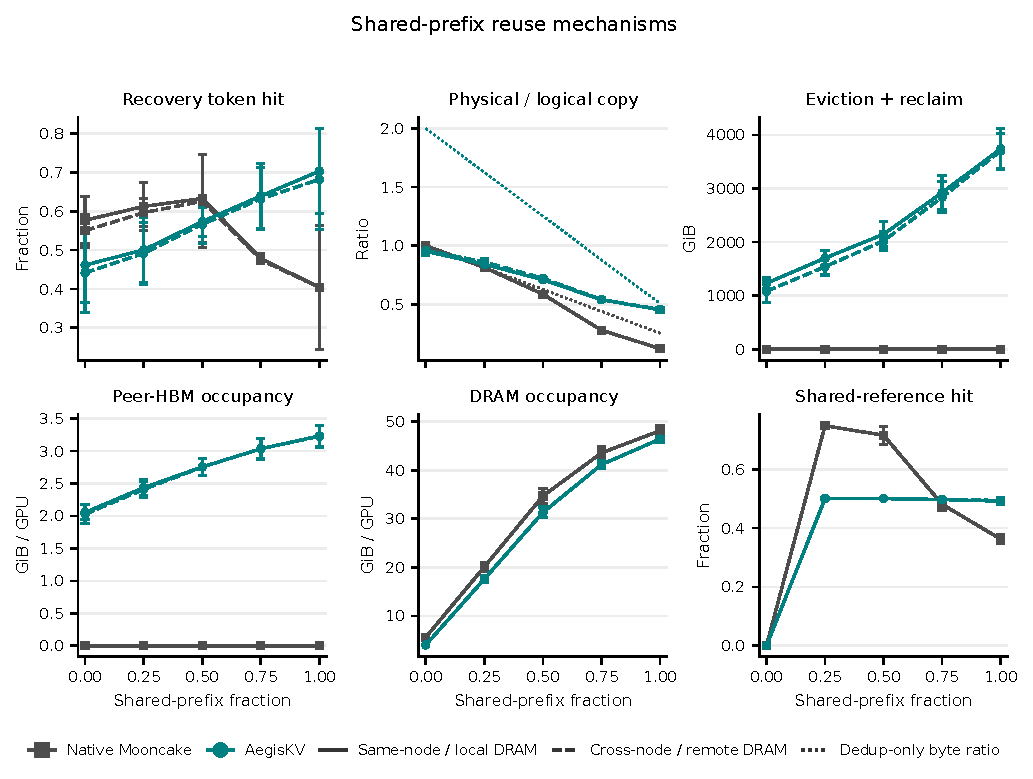
\includegraphics[width=\textwidth]{s6.pdf}
  \Description{Shared-prefix reuse mechanisms, copy amplification, and tier occupancy.}
  \caption{\textbf{S6.} Shared-prefix reuse mechanisms. Stable content identity and per-tier epochs reduce physical copies while retaining more reusable data, so lower copy amplification and higher occupancy are compatible. Sixty modeled cells, three paired seeds.}
\end{figure*}
\clearpage

\begin{figure*}[p]
  \centering
  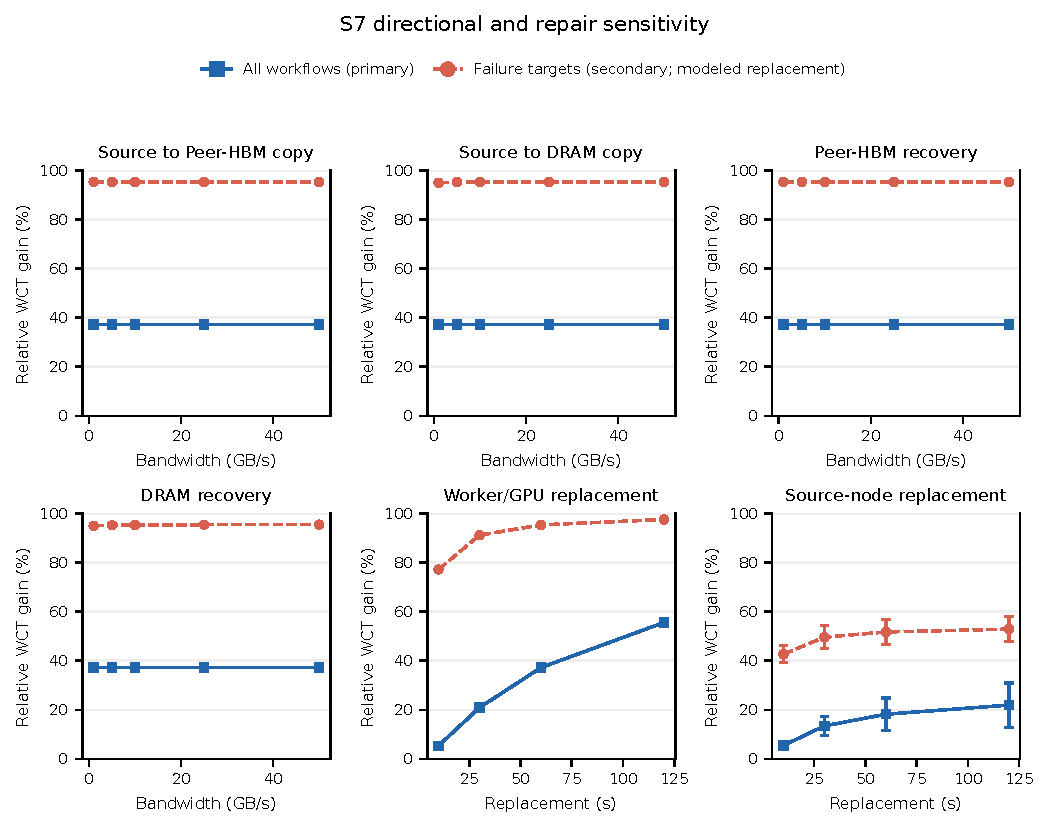
\includegraphics[width=\textwidth]{s7.pdf}
  \Description{Directional bandwidth and repair sensitivity.}
  \caption{\textbf{S7.} Directional bandwidth and repair sensitivity. Asynchronous off-path copies make bandwidth effects nearly flat, whereas modeled replacement time drives repair sensitivity. All 168 cells and 2,016 frozen failure-target probes are retained.}
\end{figure*}
\clearpage

\begin{figure*}[p]
  \centering
  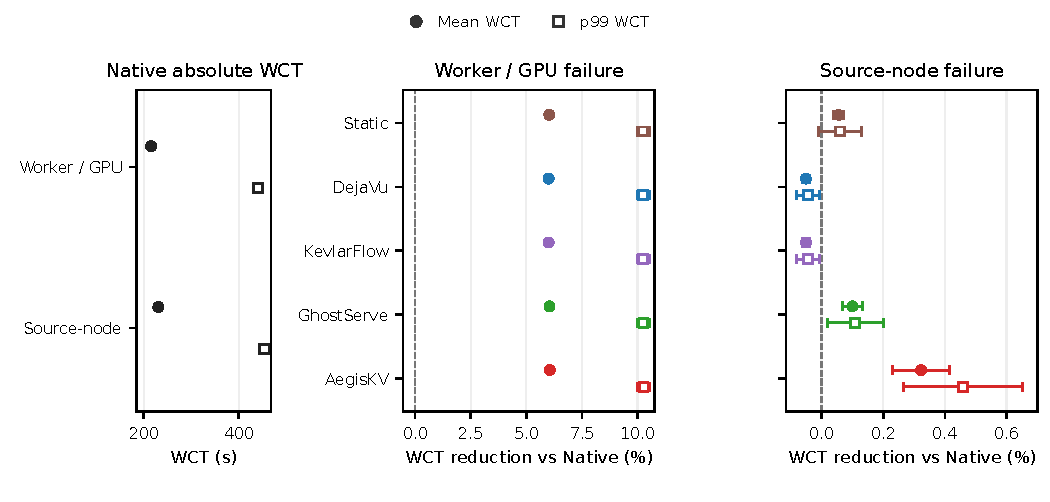
\includegraphics[width=\textwidth]{s8.pdf}
  \Description{Six-architecture comparison under Worker GPU and source-node failures.}
  \caption{\textbf{S8.} Six-architecture comparison under Worker/GPU and source-node failures. The node fault removes same-node replicas and yields much smaller gains. This view is derived from the same ten-seed sample as S1, not an independent replication.}
\end{figure*}
\clearpage

\begin{figure*}[p]
  \centering
  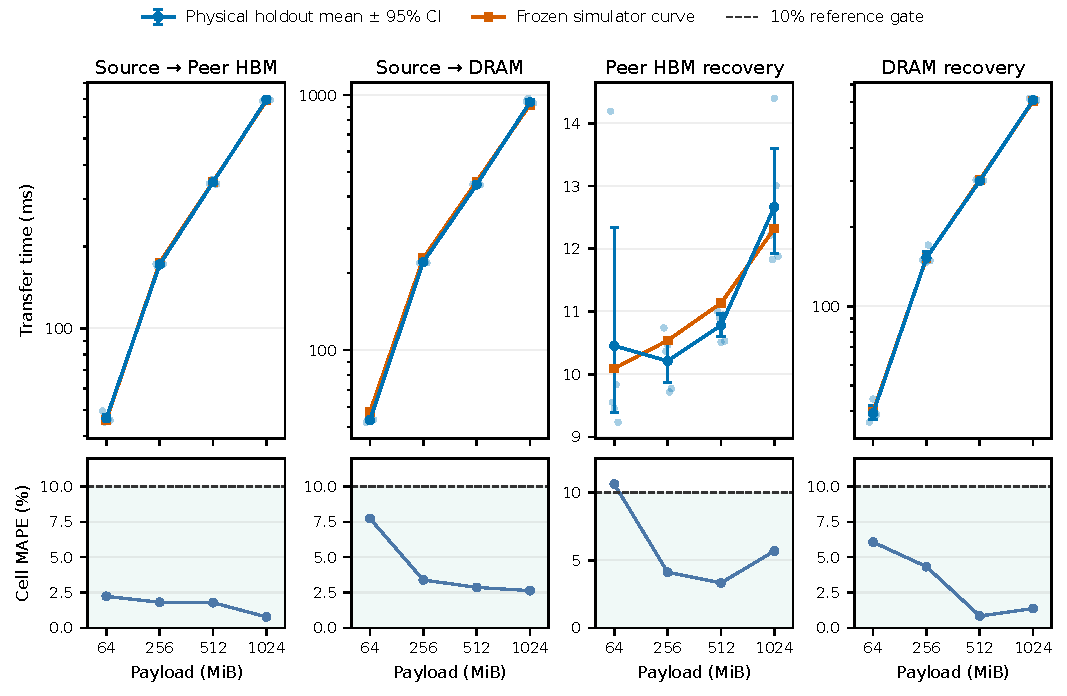
\includegraphics[width=\textwidth]{s9.pdf}
  \Description{Independent RTX4090 calibration holdout for the simulator timing model.}
  \caption{\textbf{S9.} Independent RTX4090 calibration holdout. Curves fit only on job 141298 achieve 3.72 percent overall MAPE on all 80 job-141411 samples; 15 of 16 cells meet 10 percent, while 64 MiB Peer-HBM recovery reaches 10.64 percent. No refit or exclusion.}
\end{figure*}
\clearpage

\end{document}
